\chapter{Quantization}
\label{chapter:quantization}

\abstract{
In a vector retrieval system, it is usually not enough to process queries as fast
as possible. It is equally as important to reduce the size of the index
by compressing vectors. Compression, however, must be done in such a way
that either decompressing the vectors during retrieval incurs a negligible cost, or
distances can be computed (approximately) in the compressed domain,
rendering it unnecessary to decompress compressed vectors during retrieval.
This chapter introduces a class of vector compression algorithms,
known as quantization, that is inspired by clustering.
}

\section{Vector Quantization}

Let us take a step back and present a different mental model of the clustering-based retrieval framework
discussed in Chapter~\ref{chapter:ivf}.
At a high level, we band together points that are placed by $\zeta(\cdot)$ into cluster $i$
and represent that group by $\mu_i$, for $i \in [C]$. In the first stage of the search for query $q$,
we take the following conceptual step:
First, we compute $\delta(q, \mu_i)$ for every $i$ and construct a ``table''
that maps $i$ to $\delta(q, \mu_i)$. We next approximate $\delta(q, u)$ for every $u \in \mathcal{X}$
using the resulting table: If $u \in \zeta^{-1}(i)$, then we look up an estimate of
its distance to $q$ from the $i$-th row of the table.
We then identify the $\ell$ closest distances, and perform a secondary search over
the corresponding vectors.

This presentation of clustering for top-$k$ retrieval highlights an important fact that does
not come across as clearly in our original description of the algorithm:
We have made an implicit assumption that $\delta(q, u) \approx \delta(q, \mu_i)$
for all $u \in \zeta^{-1}(i)$.
That is why we presume that if a cluster minimizes $\delta(q, \cdot)$, then the points within it
are also likely to minimize $\delta(q, \cdot)$.
That is, in turn, why we deem it sufficient to search over the points within the top-$\ell$ clusters.

Put differently, within the first stage of search, we appear to be approximating every point
$u \in \zeta^{-1}(i)$ with $\tilde{u} = \mu_i$. Because there are $C$ discrete choices to consider
for every data point, we can say that we \emph{quantize} the vectors into $[C]$.
Consequently, we can encode each vector using only
$\log_2 C$ bits, and an entire collection of vectors using $m \log_2 C$ bits!
All together, we can represent a collection $\mathcal{X}$ using $\mathcal{O}(Cd + m \log_2 C)$ space,
and compute distances to a query by performing $m$ look-ups into a table
that itself takes $\mathcal{O}(Cd)$ time to construct.
That quantity can be far smaller than $\mathcal{O}(md)$ given by the na\"ive distance computation
algorithm.

Clearly, the approximation error, $\lVert u - \tilde{u} \rVert$, is a function of $C$.
As we increase $C$, this approximation improves, so that $\lVert u - \tilde{u} \rVert \rightarrow 0$
and $\lvert \delta(q, u) - \delta(q, \tilde{u}) \rvert \rightarrow 0$.
Indeed, $C = m$ implies that $\tilde{u}=u$ for every $u$.
But increasing $C$ results in an increased space complexity and a less efficient distance computation.
At $C = m$, for example, our table-building exercise does not help speed up
distance computation for individual data points---because we
must construct the table in $\mathcal{O}(md)$ time anyway.
Finding the right $C$ is therefore critical
to space- and time-complexity, as well as the approximation or quantization error.

\subsection{Codebooks and Codewords}
What we described above is known as vector quantization~\citep{Gray1998Quantization}
for vectors in the $L_2$ space. We will therefore assume that $\delta(u, v) = \lVert u - v \rVert_2^2$
in the remainder of this section.
The function $\zeta: \mathbb{R}^d \rightarrow [C]$ is called a \emph{quantizer},
the individual centroids are referred to as \emph{codewords}, and the set of $C$
codewords make up a \emph{codebook}. It is easy to see that the set $\zeta^{-1}(i)$
is the intersection of $\mathcal{X}$ with the Voronoi region associated with codeword $\mu_i$.

The approximation quality of a given codebook is measured by the familiar mean squared error:
$\ev [\lVert \mu_{\zeta(U)} - U \rVert^2_2)]$, with $U$ denoting a random vector.
Interestingly, that is exactly the objective
that is minimized by Lloyd's algorithm for KMeans clustering. As such, an optimal codebook
is one that satisfies Lloyd's optimality conditions: each data point must be quantized to its
nearest codeword, and each Voronoi region must be represented by its mean. That is why
KMeans is our default choice for $\zeta$.

\section{Product Quantization}

As we noted earlier, the quantization error is a function of the number of clusters, $C$:
A larger value of $C$ drives down the approximation error, making the quantization
and the subsequent top-$k$ retrieval solution more accurate and effective.
However, realistically, $C$ cannot become too large, because then the framework
would collapse to exhaustive search, degrading its efficiency.
How may we reconcile the two seemingly opposing forces?

\cite{pq} gave an answer to that question in the form of Product Quantization (PQ).
The idea is easy to describe at a high level:
Whereas in vector quantization we quantize the entire vector
into one of $C$ clusters, in PQ we break up a vector into orthogonal subspaces
and perform vector quantization on individual chunks separately.
The quantized vector is then a concatenation of the quantized subspaces.

Formally, suppose that the number of dimensions $d$ is divisible by $d_\circ$,
and let $L = d/d_\circ$. Define a selector matrix $S_i \in \{0, 1\}^{d_\circ \times d}$, $1 \leq i \leq L$
as a matrix with $L$ blocks in $\{0, 1\}^{d_\circ \times d_\circ}$, where all blocks are $0$
but the $i$-th block is the identity.
The following is an example for $d = 6$, $d_\circ = 2$, and $i = 2$:
\begin{equation*}
    S_2 = 
    \begin{bmatrix}
        0 & 0 & 1 & 0 & 0 & 0 \\
        0 & 0 & 0 & 1 & 0 & 0
    \end{bmatrix}
\end{equation*}

For a given vector $u \in \mathbb{R}^d$, $S_i u$ gives the $i$-th $d_\circ$-dimensional subspace,
so that we can write: $u = \bigoplus_i\; S_i u$.
Suppose further that we have $n$ quantizers $\zeta_1$ through $\zeta_L$,
where $\zeta_i: \mathbb{R}^{d_\circ} \rightarrow [C]$ maps the subspace selected
by $S_i$ to one of $C$ clusters. Each $\zeta_i$ gives us $C$ centroids $\mu_{i,j}$
for $j \in [C]$.

Using the notation above, we can express the PQ code for a vector $u$ as $L$
cluster identifiers, $\zeta_i(S_i u)$, for $i \in [L]$. We can therefore quantize
a $d$-dimensional vector using $L \log_2 C$ bits. Observe that, when $L = 1$ (or equivalently,
$d_\circ = d$), PQ reduces to vector quantization. When $L = d$, on the other hand,
PQ performs scalar quantization per dimension.

Given this scheme, our approximation of $u$ is $\tilde{u} = \bigoplus_i \mu_{i, \zeta_i(u)}$.
It is easy to see that the quantization error $\ev[\lVert U - \tilde{U} \rVert_2^2]$, with $U$
denoting a random vector drawn from $\mathcal{X}$ and $\tilde{U}$ its reconstruction, is
the sum of the quantization error of individual subspaces:
\begin{align*}
    \ev[\lVert U - \tilde{U} \rVert_2^2] &=
        \frac{1}{m} \sum_{u \in \mathcal{X}} \Big[ \lVert u - \bigoplus_{i=1}^{L} \mu_{i, \zeta_i(u)} \rVert_2^2 \Big] \\
        &= \frac{1}{m} \sum_{u \in \mathcal{X}} \Big[ \sum_{i=1}^{L} \lVert S_i u - \mu_{i, \zeta_i(u)} \rVert_2^2 \Big].
\end{align*}
As a result, learning the $L$ codebooks can be formulated as $L$ independent
sub-problems. The $i$-th codebook can therefore be learnt by
the application of KMeans on $S_i \mathcal{X} = \{ S_i u \;|\; u \in \mathcal{X} \}$.

\subsection{Distance Computation with PQ}
In vector quantization, computing the distance of a vector $u$ to a query $q$
was fairly trivial. All we had to do was to precompute a table that maps
$i \in [C]$ to $\lVert q - \mu_i \rVert_2$, then look up the entry that corresponds to $\zeta(u)$.
The fact that we were able to precompute $C$ distances once per query, then simply look up
the right entry from the table for a vector $u$ helped us save a great deal of computation.
Can we devise a similar algorithm given a PQ code?

The answer is yes. Indeed, that is why PQ has proven to be an efficient
algorithm for distance computation. As in vector quantization, it first computes
$L$ distance tables, but the $i$-th table maps $j \in [C]$ to $\lVert S_i q - \mu_{i,j} \rVert_2^2$
(note the \emph{squared} $L_2$ distance). Using these tables, we can estimate the distance
between $q$ and any vector $u$ as follows:
\begin{align*}
    \lVert q - u \rVert_2^2 &\approx \lVert q - \tilde{u} \rVert_2^2 \\
    &= \lVert q - \bigoplus_{i=1}^L \mu_{i, \zeta_i(u)} \rVert_2^2 \\
    &= \lVert \bigoplus_{i = 1}^L \Big( S_i q - \mu_{i, \zeta_i(u)} \Big) \rVert_2^2 \\
    &= \sum_{i = 1}^L \lVert S_i q - \mu_{i, \zeta_i(u)} \rVert_2^2.
\end{align*}
Observe that, we have already computed the summands and recorded them in the distance tables.
As a result, approximating the distance between $u$ and $q$ amounts to $L$ table look-ups.
The overall amount of computation needed to approximate distances between $q$ and
$m$ vectors in $\mathcal{X}$ is then $\mathcal{O}(LCd_\circ + mL)$.

\bigskip

We must remark on the newly-introduced parameter $d_\circ$.
Even though in the context of vector quantization, the impact of $C$
on the quantization error is not theoretically known, there is nonetheless
a clear interpretation: A larger $C$ leads to better quantization.
In PQ, the impact of $d_\circ$ or, equivalently, $L$ on the quantization error
is not as clear. As noted earlier, we can say something about $d_\circ$ at the extremes,
but what we should expect from a value somewhere between $1$ and $d$ is largely
an empirical question~\citep{sun2023automating}.

\subsection{Optimized Product Quantization}
In PQ, we allocate an equal number of bits ($\log_2 C$) to each of the $n$ orthogonal subspaces.
This makes sense if our vectors have similar energy in every subspace.
But when the dimensions in one subspace are highly correlated, and in another
uncorrolated, our equal-bits-per-subspace allocation policy proves wasteful in the former
and perhaps inadequate in the latter. How can we ensure a more balanced energy across subspaces?

\cite{pq} argue that applying a random rotation $R \in \mathbb{R}^{d \times d}$ ($RR^T = I$)
to the data points prior to quantization is one way to reduce the correlation between dimensions.
The matrix $R$ together with $S_i$'s, as defined above, determines how we decompose the vector
space into its subspaces. By applying a rotation first, we no longer chunk up an input vector
into sub-vectors that comprise of consecutive dimensions.

Later,~\cite{opq} and~\cite{norouzi2013ckmeans} extended this idea and suggested that the matrix
$R$ can be learnt jointly with the codebooks. This can be done through an iterative algorithm
that switches between two steps in each iteration. In the first step, we freeze $R$ and learn
a PQ codebook as before. In the second step, we freeze the codebook and update the matrix $R$
by solving the following optimization problem:
\begin{align*}
    \min_R &\sum_{u \in \mathcal{X}} \lVert Ru - \tilde{u} \rVert_2^2, \\
    \mathit{s.t.} & \quad RR^T = I,
\end{align*}
where $\tilde{u}$ is the approximation of $u$ according to the frozen PQ codebook.
Because $u$ and $\tilde{u}$ are fixed in the above optimization problem,
we can rewrite the objective as follows:
\begin{align*}
    \min_R & \lVert RU - \tilde{U} \rVert_F, \\
    \mathit{s.t.} & \quad RR^T = I,
\end{align*}
where $U$ is a $d$-by-$m$ matrix where each column is a vector in $\mathcal{X}$,
$\tilde{U}$ is a matrix where each column is an approximation of the corresponding
column in $U$, and $\lVert \cdot \rVert_F$ is the Frobenius norm.
This problem has a closed-form solution as shown by~\cite{opq}.

\subsection{Extensions}

Since the study by~\cite{pq}, many variations of the idea have emerged in
the literature. In the original publication, for example,~\cite{pq}
used PQ codes in conjunction with the clustering-based retrieval framework presented earlier
in this chapter. In other words, a collection $\mathcal{X}$ is first clustered
into $C$ clusters (``coarse-quantization''), and each cluster
is subsequently represented using its own PQ codebook.
In this way, when the routing function identifies a cluster to search,
we can compute distances for data points within that cluster using their PQ codes.
Later,~\cite{invertedMultiIndex} extended this two-level quantization further
by introducing the ``inverted multi-index'' structure.

When combining PQ with clustering or coarse-quantization, instead of producing
PQ codebooks for raw vectors within each cluster, one could learn codebooks
for the \emph{residual} vectors instead. That means, if the centroid of the
$i$-th cluster is $\mu_i$, then we may quantize $(u - \mu_i)$ for each
vector $u \in \zeta^{-1}(i)$. This was the idea first introduced by~\cite{pq},
then developed further in subsequent works~\citep{locallyOptimizedPQ,multiscaleQuantization}.

The PQ literature does not end there. In fact, so popular, effective, and efficient is PQ
that it pops up in many different contexts and a variety of applications. Research into improving
its accuracy and speed is still ongoing. For example, there have been many works that speed
up the distance computation with PQ codebooks by leveraging hardware capabilities~\citep{pqWithGPU,Andre_2021,pqCacheLocality}.
Others that extend the algorithm to streaming (online) collections~\citep{onlinePQ},
and yet other studies that investigate other PQ
codebook-learning protocols~\citep{deepPQ,Yu_2018_ECCV,chen2020DifferentiablePQ,Jang_2021_ICCV,Klein_2019_CVPR,lu2023differeitableOPQ}.
This list is certainly not exhaustive and is still growing.

\section{Additive Quantization}

PQ remains the dominant quantization method for top-$k$ retrieval due to its overall simplicity
and the efficiency of its codebook learning protocol. There are, however, numerous generalizations of the
framework~\citep{additiveQuantization,chen2010approximate,Niu2023RVPQ,liu2015improvedRVQ,Ozan2016CompetitiveQuantization,krishnan2021projective}.
Typically, these generalized forms improve the approximation error but require more involved
codebook learning algorithms and vector encoding protocols. In this section, we review
one key algorithm, known as Additive Quantization (AQ)~\citep{additiveQuantization},
that is the backbone of all other methods.

Like PQ, AQ learns $L$ codebooks where each codebook consists of $C$ codewords.
Unlike PQ, however, each codeword is a vector in $\mathbb{R}^d$---rather than $\mathbb{R}^{d_\circ}$.
Furthermore, a vector $u$ is approximated as the \emph{sum}, instead of the concatenation,
of $L$ codewords, one from each codebook: $\tilde{u} = \sum_{i=1}^L \mu_{i, \zeta_i(u)}$,
where $\zeta_{i}: \mathbb{R}^d \rightarrow [C]$ is the quantizer associated with the
$i$-th codebook.

Let us compare AQ with PQ at a high level and understand how AQ is different.
We can still encode a data point using $L \log_2 C$ bits, as in PQ.
However, the codebooks for AQ are $L$-times larger than their PQ counterparts,
simply because each codeword has $d$ dimensions instead of $d_\circ$.
On the other hand, AQ does not decompose the space into orthogonal subspaces
and, as such, makes no assumptions about the independence between subspaces.

AQ is therefore a strictly more general quantization method than PQ.
In fact, the class of additive quantizers contains the class of product quantizers:
By restricting the $i$-th codebook in AQ to the set of codewords that are $0$
everywhere outside of the $i$-th ``chunk,'' we recover PQ.
Empirical comparisons~\citep{additiveQuantization,Matsui2018PQSurvey} confirm
that such a generalization is more effective in practice.

For this formulation to be complete, we have to specify how the codebooks are learnt,
how we encode an arbitrary vector, and how we perform distance computation.
We will cover these topics in reverse order in the following sections.

\subsection{Distance Computation with AQ}
Suppose for the moment that we have learnt AQ codebooks for a collection $\mathcal{X}$
and that we are able to encode an arbitrary vector into an AQ code (i.e.,
a vector of $L$ codeword identifiers). In this section, we examine how
we may compute the distance between a query point $q$ and a data point $u$
using its approximation $\tilde{u}$.

Observe the following fact:
\begin{equation*}
    \lVert q - u \rVert_2^2 = \lVert q \rVert_2^2 - 2 \langle q, u \rangle + \lVert u \rVert_2^2.
\end{equation*}
The first term is a constant that can be computed once per query and, at any rate,
is inconsequential to the top-$k$ retrieval problem. The last term, $\lVert u \rVert_2^2$
can be stored for every vector and looked up during distance computation,
as suggested by~\cite{additiveQuantization}. That means, the encoding of a vector
$u \in \mathcal{X}$ comprises of two components: $\tilde{u}$ and its (possibly scalar-quantized)
squared norm. This brings the total space required to encode $m$ vectors
to $\mathcal{O}(LCd + m (1 + L\log_2 C))$.

The middle term can be approximated by $\langle q, \tilde{u} \rangle$
and can be expressed as follows:
\begin{equation*}
    \langle q, u \rangle \approx \langle q, \tilde{u} \rangle =
    \sum \langle q, \mu_{i, \zeta_i(u)} \rangle.
\end{equation*}
As in PQ, the summands can be computed once for all codewords, and stored in a table.
When approximating the inner product, we can do as before and look up
the appropriate entries from these precomputed tables.
The time complexity of this operation is therefore $\mathcal{O}(LCd + mL)$
for $m$ data points, which is similar to PQ.

\subsection{AQ Encoding and Codebook Learning}
While distance computation with AQ codes is fairly similar to the process
involving PQ codes, the encoding of a data point is substantially different
and relatively complex in AQ. That is because we can no longer simply assign
a vector to its nearest codeword. Instead, we must find an arrangement of
$L$ codewords that together minimize the approximation error
$\lVert u - \tilde{u} \rVert_2$.

Let us expand the expression for the approximation error as follows:
\begin{align*}
    \lVert u - \tilde{u} \rVert_2^2 &= 
        \lVert u - \sum_{i = 1}^L \mu_{i, \zeta_i(u)} \rVert_2^2 \\
        &= \lVert u \rVert_2^2 - 2 \langle u, \sum_{i = 1}^L \mu_{i, \zeta_i(u)} \rangle + \lVert \sum_{i = 1}^L \mu_{i, \zeta_i(u)} \rVert_2^2 \\
        &= \lVert u \rVert_2^2 + \Big( \sum_{i = 1}^L - 2 \langle u, \mu_{i, \zeta_i(u)} \rangle + \lVert \mu_{i, \zeta_i(u)} \rVert_2^2 \Big) + \\
        &\quad \quad \sum_{1 \leq i < j \leq L} 2 \langle \mu_{i, \zeta_i(u)}, \mu_{j, \zeta_j(u)} \rangle.
\end{align*}
Notice that the first term is irrelevant to the objective function, so we may ignore it.
We must therefore find $\zeta_i$'s that minimize the remaining terms.

\cite{additiveQuantization} use a generalized Beam search to solve this optimization problem. 
The algorithm begins by selecting $L$ closest codewords from
$\bigcup_{i=1}^L \{ \mu_{i,1} \ldots \mu_{i,C} \}$ to $u$.
For a chosen codeword $\mu_{k,j}$, we compute the residual $u - \mu_{k,j}$
and find the $L$ closest codewords to it from $\bigcup_{i \neq k} \{ \mu_{i,1} \ldots \mu_{i,C} \}$.
After performing this search for all chosen codewords from the first round,
we end up with a maximum of $L^2$ unique pairs of codewords.
Note that, each pair has codewords from two different codebooks.

Of the $L^2$ pairs, the algorithm picks the top $L$ that minimize the approximation error.
It then repeats this process for a total of $L$ rounds, where in each
round we compute the residuals given $L$ tuples of codewords,
and for each tuple, find $L$ codewords from the remaining codebooks,
and ultimately identify the top $L$ tuples from the $L^2$ tuples.
At the end of the $L$-th round, the tuple with the minimal approximation error
is the encoding for $u$.

\bigskip

Now that we have addressed the vector encoding part, it remains to
describe the codebook learning procedure. Unsurprisingly, learning a codebook
is not so dissimilar to the PQ codebook learning algorithm.
It is an iterative procedure alternating between two steps to optimize
the following objective:
\begin{equation*}
    \min_{\mu_{i,j}} \sum_{u \in \mathcal{X}} \lVert u - \sum_{i=1}^L \mu_{i, \zeta_i(u)} \rVert_2^2.
\end{equation*}

One step of every iteration freezes the codewords and performs assignments $\zeta_i$'s,
which is the encoding problem we have already discussed above. The second step freezes
the assignments and updates the codewords, which itself is a least-squares problem
that can be solved relatively efficiently, considering that it decomposes over each dimension.

\section{Quantization for Inner Product}

The vector quantization literature has largely been focused on the Euclidean distance
and the approximate nearest neighbor search problem. Those ideas typically port over to
the maximum cosine similarity search with little effort, but not to MIPS under general conditions.
To understand why, suppose we wish to find a quantizer such that the 
inner product approximation error is minimized for a query distribution:
\begin{align*}
    \ev_{q} \Big[ \sum_{u \in \mathcal{X}} \big( \langle q, u \rangle - \langle q, \tilde{u} \rangle \big)^2 \Big] &= \sum_{u \in \mathcal{X}} \ev_q \Big[ \langle q, u - \tilde{u} \rangle^2 \Big] \\
    &= \sum_{u \in \mathcal{X}} \ev_q \Big[ (u - \tilde{u})^T qq^T (u - \tilde{u}) \Big] \\
    &= \sum_{u \in \mathcal{X}} (u - \tilde{u})^T \ev_q \big[ qq^T \big] (u - \tilde{u})
    \numberthis \label{equation:quantization:mips-objective},
\end{align*}
where $\tilde{u}$ is an approximation of $u$.
If we assumed that $q$ is isotropic, so that its covariance matrix is the identity matrix
scaled by some constant,
then the objective above reduces to the reconstruction error. In that particular case,
it makes sense for the quantization objective to be based on the reconstruction error,
making the quantization methods we have studied thus far appropriate for MIPS too.
But in the more general case, where the distribution of $q$ is anisotropic, there is
a gap between the true objective and the reconstruction error.

\cite{guo2016Quip} showed that, if we are able to obtain a small sample of queries
to estimate $\ev[qq^T]$, then we can modify the assignment step in
Lloyd's iterative algorithm for KMeans in order to minimize the objective in
Equation~(\ref{equation:quantization:mips-objective}).
That is, instead of assigning points to clusters by their Euclidean distance to 
the (frozen) centroids, we must instead use Mahalanobis distance characterized by
$\ev[qq^T]$. The resulting quantizer is arguably more suitable for inner product
than the plain reconstruction error.

\subsection{Score-aware Quantization}

Later,~\cite{scann} argued that the objective in Equation~(\ref{equation:quantization:mips-objective})
does not adequately capture the nuances of MIPS. Their argument rests on an observation and an intuition.
The observation is that, in Equation~(\ref{equation:quantization:mips-objective}), every single
data point contributes equally to the optimization objective. Intuitively, however,
data points are not equally likely to be the solution to MIPS.
The error from data points that are more likely to be the maximizers of inner product
with queries should therefore be weighted more heavily than others.

On the basis of that argument,~\cite{scann} introduce the following objective
for inner product quantization:
\begin{equation}
    \label{equation:quantization:scann-objective}
    \sum_{u \in \mathcal{X}} \underbrace{\ev_q \Big[  \omega(\langle q, u \rangle) \;
    \langle q, u - \tilde{u} \rangle^2 \Big]}_{\ell(u, \tilde{u}, \omega)}.
\end{equation}
In the above, $\omega: \mathbb{R} \rightarrow \mathbb{R}^+$ is an arbitrary weight function
that determines the importance of each data point to the optimization objective.
Ideally, then, $\omega$ should be monotonically non-decreasing in its argument.
One such weight function is $\omega(s) = \mathbbm{1}_{s \geq \theta}$ for some threshold $\theta$,
implying that only data points whose expected inner product is at least $\theta$ contribute to the
objective, while the rest are simply ignored. That is the weight function that~\cite{scann}
choose in their work.

\medskip

Something interesting emerges from Equation~(\ref{equation:quantization:scann-objective}) with the choice
of $\omega(s) = \mathbbm{1}_{s \geq \theta}$: It is more important for $\tilde{u}$ to preserve the
\emph{norm} of $u$ than it is to preserve its \emph{angle}. We will show why that is shortly, but
consider for the moment the reason this behavior is important for MIPS.
Suppose there is a data point whose norm is much larger than the rest of the data points.
Intuitively, such a data point has a good chance of maximizing inner product
with a query even if its angle with the query is relatively large.
In other words, being a candidate solution to MIPS is less sensitive to angles and more sensitive
to norms. Of course, as norms become more and more concentrated, angles take on a bigger role in determining
the solution to MIPS. So, intuitively, an objective that penalizes the distortion of norms more than
angles is more suitable for MIPS.

\subsubsection{Parallel and Orthogonal Residuals}

\begin{figure}[t]
    \centering
    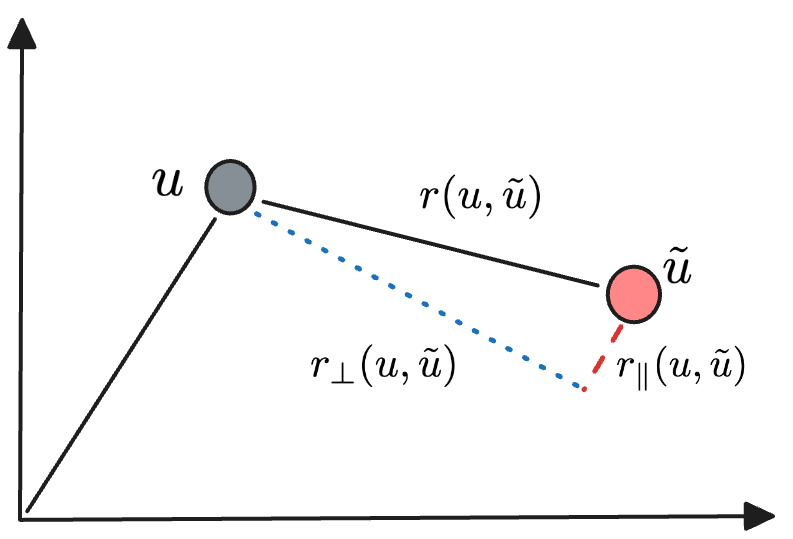
\includegraphics[width=0.4\linewidth]{figures/clustering-residual-error-decomposition.png}
    \caption{Decomposition of the residual error $r(u, \tilde{u}) = u - \tilde{u}$ for $u \in \mathbb{R}^2$
    to one component that is \emph{parallel} to the data point, $r_\parallel(u, \tilde{u})$,
    and another that is \emph{orthogonal} to it, $r_\perp(u, \tilde{u})$.}
    \label{figure:quantization:residual-error-decomposition}
\end{figure}

Let us present this phenomenon more formally and show why the statement above is true.
Define the residual error as $r(u, \tilde{u}) = u - \tilde{u}$.
The residual error can be decomposed into two components: one that is parallel to the
data point, $r_{\parallel}(u, \tilde{u})$, and another that is orthogonal to it, $r_\perp(u, \tilde{u})$,
as depicted in Figure~\ref{figure:quantization:residual-error-decomposition}.
More concretely:
\begin{equation*}
    r_\parallel(u, \tilde{u}) = \frac{ \langle u - \tilde{u}, u \rangle}{\lVert u \rVert^2}\; u,
\end{equation*}
and,
\begin{equation*}
    r_\perp(u, \tilde{u}) = r(u, \tilde{u}) - r_\parallel(u, \tilde{u}).
\end{equation*}

\cite{scann} show first that, regardless of the choice of $\omega$, the loss
defined by $\ell(u, \tilde{u}, \omega)$ in Equation~(\ref{equation:quantization:scann-objective})
can be decomposed as stated in the following theorem.

\begin{figure}[t]
    \centering
    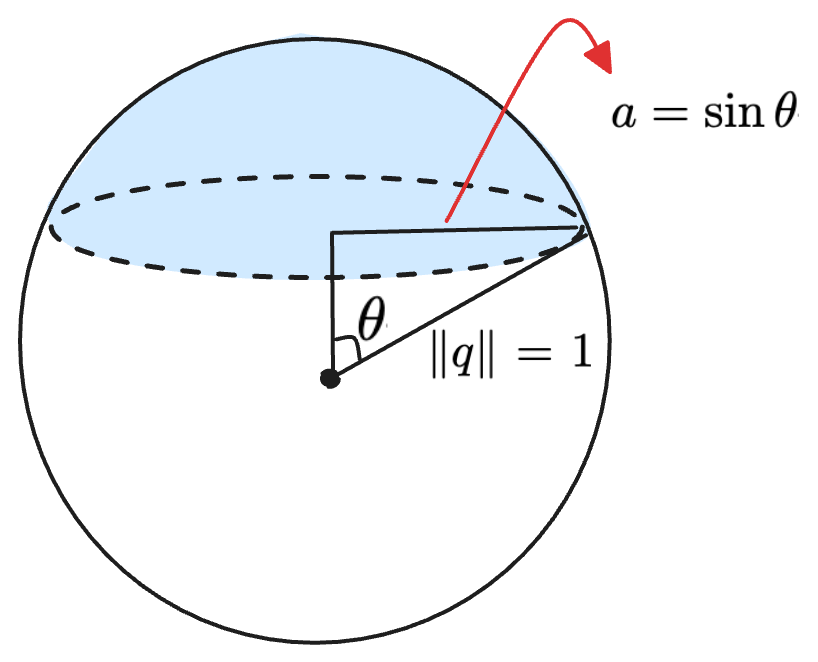
\includegraphics[width=0.4\linewidth]{figures/clustering-spherical-cap.png}
    \caption{The probability that the angle between a fixed data point $u$ with a
    unit-normed query $q$ that is drawn from a spherically-symmetric distribution is at most $\theta$,
    is equal to the surface area of the spherical cap with base radius $a = \sin \theta$. This fact
    is used in the proof of Theorem~\ref{theorem:quantization:scann:decomposition}.}
    \label{figure:quantization:spherical-cap-area}
\end{figure}

\begin{theorem}
    \label{theorem:quantization:scann:decomposition}
    Given a data point $u$, its approximation $\tilde{u}$, and any weight function $\omega$,
    the objective of Equation~(\ref{equation:quantization:scann-objective}) can be decomposed as follows
    for a spherically-symmetric query distribution:
    \begin{equation*}
        \ell(u, \tilde{u}, \omega) \propto h_\parallel(\omega, \lVert u \rVert) \; \lVert r_\parallel(u, \tilde{u}) \rVert^2 +
        h_\perp(\omega, \lVert u \rVert) \; \lVert r_\perp(u, \tilde{u}) \rVert^2,
    \end{equation*}
    where,
    \begin{equation*}
        h_\parallel(\omega, t) = \int_0^\pi \omega(t \cos \theta) \Big( \sin^{d-2}\theta - \sin^d \theta \Big) \; d\theta,
    \end{equation*}
    and,
    \begin{equation*}
        h_\perp(\omega, t) = \frac{1}{d-1} \int_0^\pi \omega(t \cos \theta) \sin^d \theta \; d\theta.
    \end{equation*}
\end{theorem}
\begin{proof}
Without loss of generality, we can assume that queries are unit vectors (i.e., $\lVert q \rVert = 1$).
Let us write $\ell(u, \tilde{u}, \omega)$ as follows:
\begin{align*}
    \ell(u, \tilde{u}, \omega) &= \ev_q \Big[ \omega(\langle q, u \rangle) \; \langle q, u - \tilde{u} \rangle^2 \Big] \\
    &= \int_0^\pi \omega(\lVert u \rVert \cos \theta) \ev_q \Big[ \langle q, u - \tilde{u} \rangle^2 \big| \langle q, u \rangle = \lVert u \rVert \cos \theta \Big] \; d \probability\Big[ \theta_{q,u} \leq \theta \Big],
\end{align*}
where $\theta_{q, u}$ denotes the angle between $q$ and $u$.

Observe that
$\probability\Big[ \theta_{q,u} \leq \theta \Big]$ is the surface area of a spherical cap with base radius
$a = \lVert q \rVert \sin \theta = \sin \theta$---see Figure~\ref{figure:quantization:spherical-cap-area}.
That quantity is equal to:
\begin{equation*}
    \lVert q \rVert^{d - 1} \frac{\pi^{d/2}}{\Gamma(d/2)} I(a^2; \frac{d-1}{2}, \frac{1}{2}),
\end{equation*}
where $\Gamma$ is the Gamma function and $I(z; \cdot, \cdot)$ is the incomplete Beta function.
We may therefore write:
\begin{align*}
    \frac{d \probability\Big[ \theta_{q,u} \leq \theta \Big]}{d \theta} &\propto \Big[ (1 - a^2)^{\frac{1}{2} - 1} (a^2)^{\frac{d - 1}{2} - 1} \Big] \frac{d a}{d \theta} \\
    &= \frac{\sin^{d-3} \theta}{\cos \theta} (2 \sin \theta \cos \theta) \\
    &\propto \sin^{d-2} \theta,
\end{align*}
where in the first step we used the fact that $d I(z; s, t) = (1 - z)^{t - 1} z^{s-1} dz$.

Putting everything together, we can rewrite the loss as follows:
\begin{equation*}
    \ell(u, \tilde{u}, \omega) \propto \int_0^\pi \omega(\lVert u \rVert \cos \theta) \ev_q \Big[ \langle q, u - \tilde{u} \rangle^2 \big| \langle q, u \rangle = \lVert u \rVert \cos \theta \Big] \sin^{d-2}\theta \; d\theta.
\end{equation*}
We can complete the proof by applying the following lemma to the expectation over queries in the integral
above.

\begin{lemma}
\begin{equation*}
    \ev_q[\langle q, u - \tilde{u} \rangle^2 \big| \langle q, u \rangle = t] = 
    \frac{t^2}{\lVert u \rVert^2} \lVert r_\parallel(u, \tilde{u}) \rVert^2 +
    \frac{1 - t^2/\lVert u \rVert^2}{d - 1} \rVert r_\perp(u, \tilde{u}) \rVert^2.
\end{equation*}
\end{lemma}
\begin{proof}
    We use the shorthand $r_\parallel = r_\parallel(u, \tilde{u})$ and similarly
    $r_\perp = r_\perp(u, \tilde{u})$.
    Decompose $q = q_\parallel + q_\perp$ where $q_\parallel = \langle q, u \rangle \frac{u}{\lVert u \rVert^2}$ and $q_\perp = q - q_\parallel$. We can now write:
    \begin{align*}
        \ev_q[\langle q, u - \tilde{u} \rangle^2 \big| \langle q, u \rangle = t] =
        \ev_q[\langle q_\parallel, r_\parallel \rangle^2] \big| \langle q, u \rangle = t] +
        \ev_q[\langle q_\perp, r_\perp \rangle^2] \big| \langle q, u \rangle = t].
    \end{align*}
    All other terms are equal to $0$ either due to orthogonality or components or because of
    spherical symmetry. The first term is simply equal to
    $\lVert r_\parallel \rVert^2 \frac{t^2}{\lVert u \rVert^2}$.
    By spherical symmetry, it is easy to show that the second term reduces to
    $\frac{1 - t^2/\lVert u \rVert^2}{d - 1} \lVert r_\perp \rVert^2$.
    That completes the proof.
\end{proof}

Applying the lemma above to the integral, we obtain:
\begin{equation*}
    \ell(u, \tilde{u}, \omega) \propto \int_0^\pi \omega(\lVert u \rVert \cos \theta) 
    \Bigg(
    \cos^2 \theta \lVert r_\parallel(u, \tilde{u}) \rVert^2 + \frac{\sin^2 \theta}{d - 1} \lVert r_\perp(u, \tilde{u}) \rVert^2
    \Bigg)
    \sin^{d-2}\theta \; d\theta,
\end{equation*}
as desired.
\end{proof}

When $\omega(s) = \mathbbm{1}_{s \geq \theta}$ for some $\theta$,~\cite{scann} show that
$h_\parallel$ outweighs $h_\perp$, as the following theorem states. This implies that
such an $\omega$ puts more emphasis on preserving the parallel residual error as discussed earlier.

\begin{theorem}
    For $\omega(s) = \mathbbm{1}_{s \geq \theta}$ with $\theta \geq 0$, $h_\parallel(\omega, t) \geq h_\perp(\omega, t)$,
    with equality if and only if $\omega$ is constant over the interval $[-t, t]$.
\end{theorem}
\begin{proof}
    We can safely assume that $h_\parallel$ and $h_\perp$ are positive; they are $0$ if and only if
    $\omega(s) = 0$ over $[-t, t]$. We can thus express the ratio between them as follows:
    \begin{equation*}
        \frac{h_\parallel(\omega, t)}{h_\perp(\omega, t)} = (d - 1)
            \Bigg( \frac{\int_0^\pi \omega(t\cos \theta) \sin^{d-2}\theta \;d\theta }{\int_0^\pi \omega(t \cos \theta) \sin^d\theta \; d\theta} - 1\Bigg) = (d - 1) \Big( \frac{I_{d-2}}{I_d} -1 \Big),
    \end{equation*}
    where we denoted by $I_d = \int_0^\pi \omega(t \cos \theta) \sin^d \theta \; d\theta$.
    Using integration by parts:
    \begin{align*}
        I_d &= - \omega(t \cos \theta) \cos \theta \sin^{d-1}\theta \Big|_0^\pi + \\
        &\int_0^\pi \cos \theta \Big[ \omega(t \cos \theta)(d-1)\sin^{d-2}\theta \cos \theta -
        \omega^\prime(t \cos \theta) t \sin^d \theta \Big] \; d\theta \\
        &= (d - 1) \int_0^\pi \omega(t \cos \theta) \cos^2 \theta \sin^{d-2}\theta \; d\theta -
        t \int_0^\pi \omega^\prime(t \cos \theta) \cos \theta \sin^d \theta \; d\theta \\
        &= (d - 1) I_{d-2} - (d - 1) I_d -
        t \int_0^\pi \omega^\prime(t \cos \theta) \cos \theta \sin^d \theta \; d\theta.
    \end{align*}
    Because $\omega(s) = 0$ for $s < 0$, the last term reduces to an integral over $[0, \pi/2]$.
    The resulting integral is non-negative because sine and cosine are both non-negative over that interval.
    It is $0$ if and only if $\omega^\prime = 0$, or equivalently when $\omega$ is constant.
    We have therefore shown that:
    \begin{equation*}
        I_d \leq (d - 1) I_{d-2} - (d-1) I_d \implies (d - 1) \Big( \frac{I_{d-2}}{I_d} - 1 \Big) \geq 1
        \implies \frac{h_\parallel(\omega, t)}{h_\perp(\omega, t)} \geq 1,
    \end{equation*}
    with equality when $\omega$ is constant, as desired.
\end{proof}

\subsubsection{Learning a Codebook}

The results above formalize the intuition that the parallel residual plays a more important
role in quantization for MIPS. If we were to plug the formalism above into the objective
in Equation~(\ref{equation:quantization:scann-objective}) and optimize it to learn a codebook, we would
need to compute $h_\parallel$ and $h_\perp$ using Theorem~\ref{theorem:quantization:scann:decomposition}.
That would prove cumbersome indeed.

Instead,~\cite{scann} show that $\omega(s) = \mathbbm{1}_{s \geq \theta}$ results in a more
computationally-efficient optimization problem. 
Letting $\eta(t) = \frac{h_\parallel(\omega, t)}{h_\perp(\omega, t)}$,
they show that $\eta/(d-1)$ concentrates around $\frac{(\theta/t)^2}{1 - (\theta/t)^2}$
as $d$ becomes larger. So in high dimensions, one can rewrite the objective function
of Equation~(\ref{equation:quantization:scann-objective}) as follows:
\begin{equation*}
    \sum_{u \in \mathcal{X}} \frac{(\theta/\lVert u \rVert)^2}{1 - (\theta/\lVert u \rVert)^2}
    \lVert r_\parallel(u, \tilde{u}) \rVert^2 +
    \lVert r_\perp(u, \tilde{u}) \rVert^2.
\end{equation*}

\cite{scann} present an optimization procedure that is based on Lloyd's iterative algorithm for
KMeans, and use it to learn a codebook by minimizing the objective above.
Empirically, such a codebook outperforms the one that
is learnt by optimizing the reconstruction error.

\subsubsection{Extensions}
The score-aware quantization loss has, since its publication, been extended
in two different ways. \cite{Zhang_Liu_Lian_Liu_Wu_Chen_2022} adapted the objective
function to an Additive Quantization form. \cite{queryAwareQuantization}
updated the weight function $\omega(\cdot)$ so that the importance of a data point
can be estimated based on a given set of training queries. Both extensions lead
to substantial improvements on benchmark datasets.

\bibliographystyle{abbrvnat}
\bibliography{biblio}
